\section{Frontend}\label{sec:frontend}

The frontend's purpose is to present the data
it got from the backend to a user
in a manner that is both easy to read
and visually attractive.
Modern frontend applications
are expected to include
fast loading times,
asynchronous data fetching,
intuitive interface,
and some degree of familiarity,
which means they have to resemble
popular services to some extent.

When designing the \ac{UI} for Notipie,
I wanted not only to deliver great visual design,
but also intuitive user experience,
reliability,
and snappiness.
The frontend code
is in the
\texttt{ui} directory~\cite{sewera_notipie_2022-5}.
The \ac{UI} is available both in dark and light mode,
as illustrated in figures~\ref{fig:notipie-ui-dark}
and~\ref{fig:notipie-ui-light} respectively.

\begin{figure}[h]
  \centering
  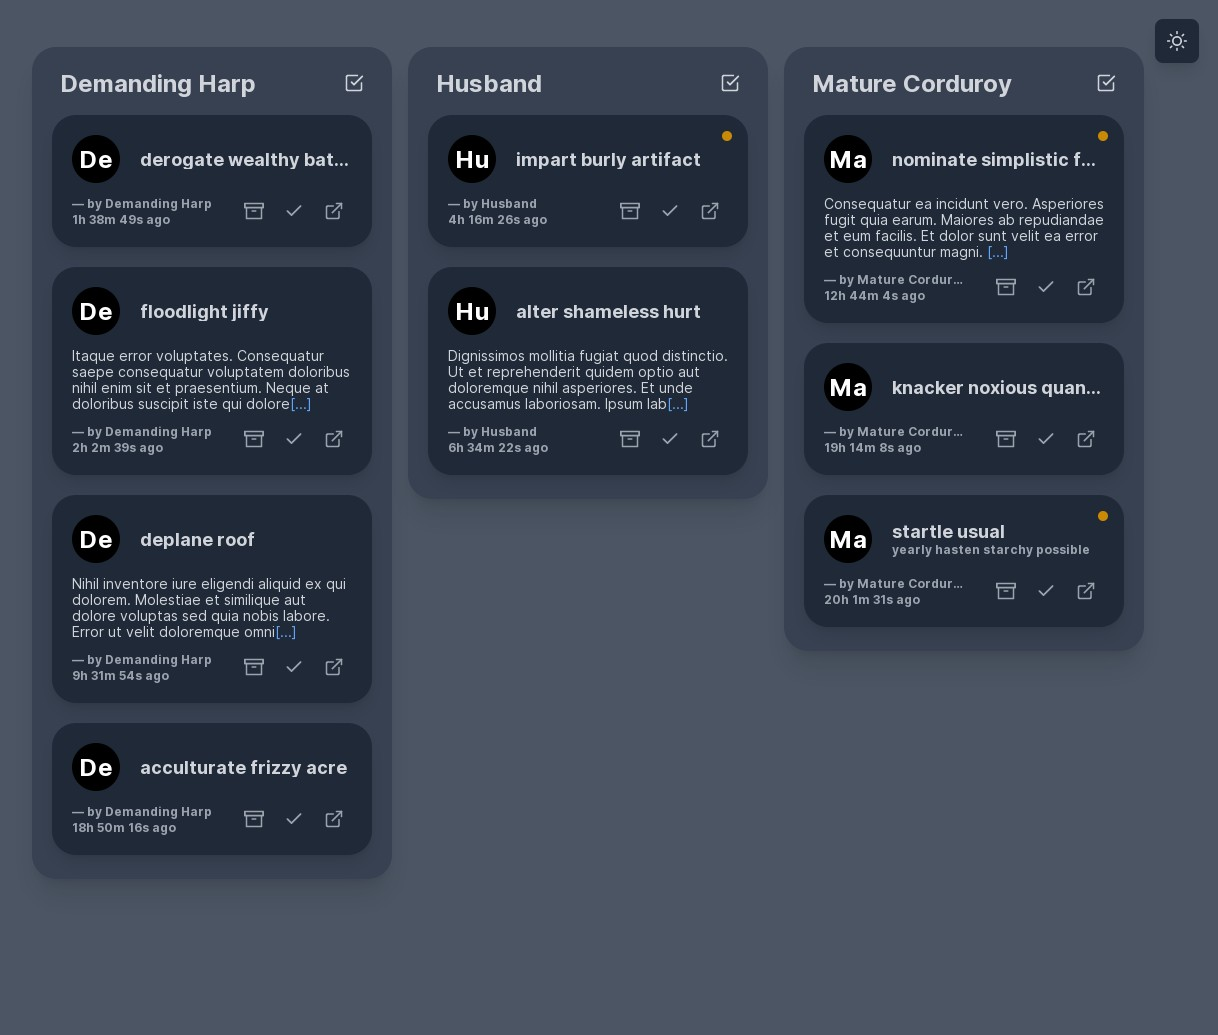
\includegraphics[width=9cm,keepaspectratio]{img/notipie_dark.jpg}
  \caption{Notipie UI: Dark mode}
  \label{fig:notipie-ui-dark}
\end{figure}

\begin{figure}[h]
  \centering
  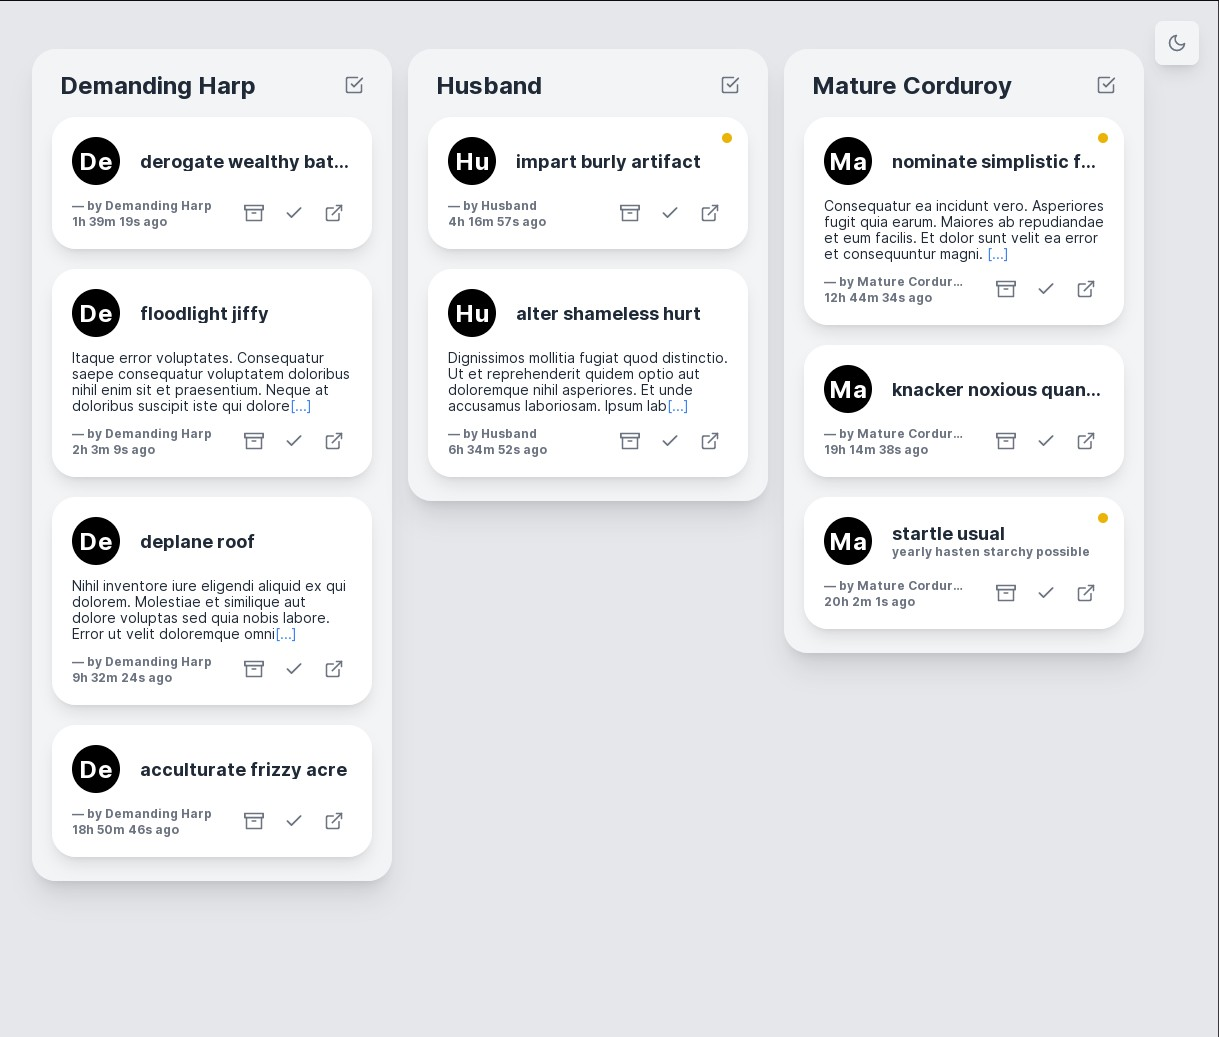
\includegraphics[width=9cm,keepaspectratio]{img/notipie_light.jpg}
  \caption{Notipie UI: Light mode}
  \label{fig:notipie-ui-light}
\end{figure}

\subsection{UI Design}\label{sec:ui-design}

When designing the UI of Notipie,
I tried to maximize usability,
and minimize complexity of the interface.
Maintaining simplicity of the interface is not an easy task,
so I took inspiration from the professional designs.

\subsubsection{Inspirations}\label{sec:inspirations}

My main inspirations for the interface were
Apple Human Interface Guidelines~\cite{apple_inc_human_2022}
and Google's Material Design~\cite{google_llc_material_2022},
but by far the most inspiration was taken from
Github Primer~\cite{github_inc_primer_2022}.
I tried to break down what is useful,
what is unnecessary in my project,
and extract only the essentials for my design.

Adam Wathan and Steve Schoger
also had a great influence
on my design decisions.
Their book,
\citetitle{wathan_refactoring_2018}~\cite{wathan_refactoring_2018}
was an excellent guidance of the best practices
of the modern user interface design.

\subsubsection{Final design}\label{sec:final-design}

\paragraph*{The card}\label{par:the-card}

The card is a building block for the entire user interface.
It provides the most interaction in the whole application,
therefore it had to be designed with clearly laid out information
and intuitive controls.
The card itself consists of several elements,
as depicted in figure~\ref{fig:card-with-labeled-elements}:

\begin{enumerate}
      \item
            logo,
            it can be an image
            or automatically generated SVG
            from the first two letters of the app's name,
      \item
            indicator,
            whether the notification has been seen or not,
      \item
            title of the notification,
      \item
            subtitle,
      \item
            body,
            that collapses after it reaches a certain length,
            so that an ellipsis appears (\texttt{...}),
      \item
            information about what app sent the notification and when it happened,
      \item
            controls to archive,
            mark as read,
            or go to external site connected with the notification,
            like a certain build on Jenkins,
            or the notification page on Github.
\end{enumerate}

The card was also designed with aesthetics in mind.
All elements were carefully positioned and aligned,
so they are not only pleasant to look at,
but also have features important for visual communication.
Those features, highlighted in figure~\ref{fig:card-with-guides}, include:

\begin{itemize}
      \item
            the rounded corners take the focus away from the card frame,
            and provide a natural, neutral enclosure for the notification,
      \item
            the inner padding is of equal size in each direction
            to provide optical stability,
      \item
            the distance between the logo and title -- subtitle combo
            is the same size as the padding,
            making the logo appear centered,
      \item
            the title -- subtitle combo itself
            is centered vertically relative to the logo,
      \item
            the distances between the logo,
            notification body, and app name -- timestamp combo are shorter
            in order to make the inner section more connected,
      \item
            the controls are centered relative to the app name -- timestamp combo,
      \item
            the \textit{unread} indicator is unobtrusive enough
            not to steal all the focus from the card's content,
      \item
            finally, the \textit{unread} indicator
            is positioned slightly outside the inner section,
            so that it belongs to the card itself,
            not its content,
            therefore it is easier to spot at a glance.
\end{itemize}

\begin{figure}[p]
      \centering
      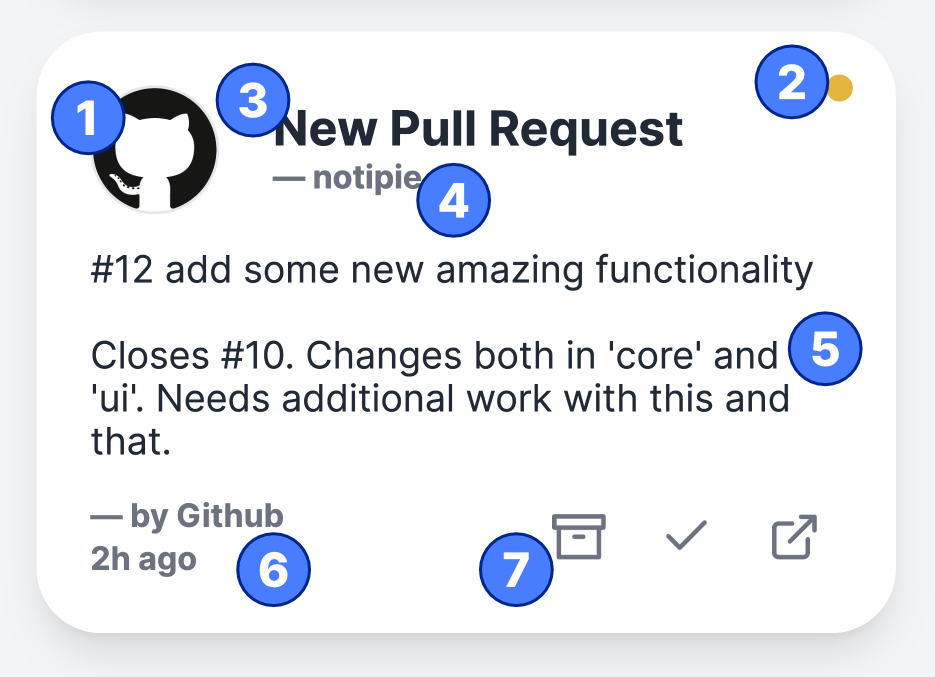
\includegraphics[width=10cm,keepaspectratio]{img/card_labeled.png}
      \caption{The card with labeled elements}
      \label{fig:card-with-labeled-elements}
\end{figure}

\begin{figure}[p]
      \centering
      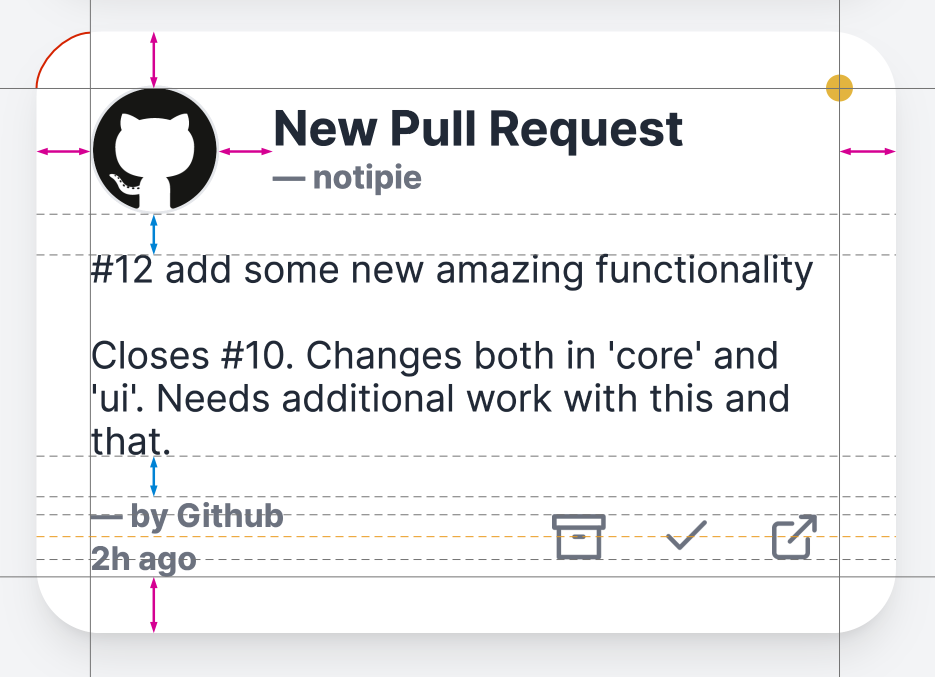
\includegraphics[width=10cm,keepaspectratio]{img/card_guides.png}
      \caption{The card with guides}
      \label{fig:card-with-guides}
\end{figure}

\subsection{UI components}\label{sec:ui-components}

Using components enabled me to split my UI
into small, reusable components,
eliminating code duplication,
and helping with maintaining the consistent look.
I wanted to choose the right library
for this task,
so that the development would be quick,
and I would have plenty of tools
that would help me achieve
good architecture for the frontend.

\subsubsection{UI component library}\label{sec:ui-component-library}

When choosing the library for the UI components, I considered:

\begin{itemize}
  \item
        React~\cite{oshannessy_react_2022},
  \item
        Vue.js~\cite{you_vuejs_2022}, and
  \item
        Angular~\cite{kalpakas_angular_2022}.
\end{itemize}

All those libraries are very popular,
so I chose React,
because I had the most experience with it in my professional work.

\subsubsection{The component directory}\label{sec:the-component-directory}

All of the frontend components
are located in the component directory~\cite{sewera_notipie_2022-3}.
The directories are divided by category.
There are currently two categories,
\emph{canvas}, and
\emph{notification}.

Canvas category includes
an \emph{AppCanvas} component,
responsible for displaying
a background in the right color,
and controlling the light or dark mode setting.

Notification category includes
a notification card\footnote{
  The design of the card
  is explained in detail
  in section~\ref{sec:final-design}.
}, a notification container,
which contains all the notifications
from the same App\footnote{
  The concept of an App is described
  in section~\ref{sec:app}.
}, and a notification board,
containing all the notifications
presented in the UI.

\subsubsection{Testing}\label{sec:ui-testing}



\subsubsection{Storybook}\label{sec:storybook}

\subsection{UI networking}\label{ui-networking}

The nature of notifications required me to use
both REST data fetching and asynchronous data pushes from the backend.
For the latter, I decided to use WebSockets,
a standard defined in RFC6455~\cite{fette_rfc6455_2011}, and
RxJS~\cite{lesh_rxjs_2022}, an implementation of
ReactiveX library~\cite{gross_reactivex_2021}.

\subsubsection{REST data fetching}\label{rest-data-fetching}

I used simple REST~\cite{perrier_rest_2022} requests
for fetching the notifications
that are already on the backend server.
The standard Fetch browser API~\cite{perrier_fetch_2022}
was sufficient for the task.

\subsubsection{Reactive Raven}\label{reactive-raven}

This project~\cite{sewera_reactive_2022} was an experiment
on using RxJS for all real-time data fetching,
enabling the separation of concerns in the code,
and decoupling the state management implementation
from the networking implementation.

When searching for the optimal solution for pushing the data to the UI,
I came across two major solutions:

\begin{itemize}
  \item
        Redux Thunk~\cite{gaeraon_redux_2022-1} --
        enough for fetching data on user interaction,
        e.g., on a button click,
        but it provides virtually full implementation lock-in
        to the Redux store, and very little separation of concerns.
        Fetching data is an action dispatched on a store,
        so external communication and storing data are dependent on each other.
  \item
        Redux Saga~\cite{elouafi_redux_2022} --
        good for managing side effects with plain JavaScript,
        but it uses generator functions
        that yield a different type every time,
        so it is very problematic to use with strict TypeScript.
\end{itemize}

Both thunks and sagas did not provide the separation of concerns
I wanted to achieve.
Fetching or acting upon pushed data
is a different concern than storing it.

As a user,
I should not have to dispatch an action on a store
when I want to fetch data.
Of course, the data can be immediately stored after fetching,
but this behavior should be injected later,
so that there is no store implementation lock-in.

This separation of concerns enabled me to
migrate from Redux to Zustand as my \emph{store} implementation,
as described in the next section.

\subsection{State management in UI}\label{sec:state-management-in-ui}

To simplify the frontend code,
I needed to use a single source of truth for the data.
I used both Redux~\cite{gaeraon_redux_2022},
and Zustand~\cite{kato_zustand_2022} for this task
as \textit{store} implementations,
and Zustand came on top as a simpler solution for my application.

\subsubsection{Redux}\label{sec:redux}

Redux is great for big applications with lots of components.
Being one of the most popular state management libraries for React,
it was my first choice.
Unfortunately,
it required me to write a lot of boilerplate code,
and thus was not easily maintainable
for a smaller project like Notipie.

\subsubsection{Zustand}\label{sec:zustand}

Zustand is a lot simpler than Redux,
requires a lot less boilerplate code,
and was sufficient for my application.
I migrated to it in commit
\texttt{7677d13}\footfullcite{sewera_choreui_2022},
and it reduced the lines of code by over 200.
I did not, however, give up the connected components,
as they provide better testability and separation of concerns,
which is worth a bit extra code.

\addtocategory{commit}{sewera_choreui_2022}

\subsection{TypeScript in UI}\label{sec:typescript-in-ui}

I decided to use TypeScript in my project for the frontend part,
because of its type checking tools,
huge popularity,
and a growing demand for in on the job market.

\subsubsection{Choosing the language}\label{sec:choosing-the-language}

When choosing which language to use in the UI,
I considered a couple of options:

\begin{itemize}
      \item
            plain JavaScript,
      \item
            TypeScript,
      \item
            Elm, and
      \item
            CoffeeScript.
\end{itemize}

I immediately discarded the last two,
due to their smaller popularity,
compared to JavaScript or TypeScript.

The featureset of the language was also very important to me.
JavaScript is by far the most popular,
but it lacks type annotations or pre-runtime type checking.
TypeScript and Elm turned out to be winners in the type checking toolchain.

TypeScript also has a big advantage of being very similar to plain JavaScript,
so the transpiled code is very readable.

A big factor was general trend of language's popularity growth.
TypeScript was a clear winner in this scenario,
being third most loved language
and second most wanted language
in the Stack Overflow Developer Survey 2021~\cite{stack_overflow_2021_2021}.

It was only beaten by Rust and Clojure
in the \textit{Most Loved} section,
both of which are non-frontend languages,
and Python in the \textit{Most Wanted} section,
which is also not a frontend language.

Another report confirming the growing popularity of TypeScript
is Github Octoverse Report 2021~\cite{github_inc_2021_2021}.
Since 2017,
it beat
Ruby,
C,
C++,
C\#,
Shell, and
PHP
and is, as of 2021, the fourth top language on Github.

\subsubsection{Working with TypeScript}\label{sec:working-with-typescript}

Starting with TypeScript was fairly easy.
The toolchain was included in the project creation scripts.
Most dependencies had good TypeScript annotations,
or they were completely written in TypeScript,
which was very helpful for maintaining type safety.

Learning the language was also very easy.
I was already familiar with JavaScript,
so I only needed to learn the type annotations,
which were very intuitive to use.

\subsection{Build system}\label{build-system}

For the build and bundle software,
I wanted to use something modern,
with hot module reloading,
easy to use setup scripts,
customizable development server,
and short bundle times.

\subsubsection{Snowpack and Vite}\label{snowpack-and-vite}

I started with Snowpack~\cite{schott_snowpack_2021}
and used it until I decided to move to Vite~\cite{you_vite_2022}
in commit \texttt{c11bc35}\footnote{
  commit \texttt{c11bc35}, 2021.
    [Online]. (visited on 2022-05-31).
  \url{https://github.com/blazejsewera/notipie/commit/c11bc35370f512f35d522a55fcd216c1c80ea75a}
}.

Snowpack offered both hot module reloading and short bundle times,
however, there were some minor problems from time to time, the project
had a slow development, and the alternative, Vite did not seem to have
those problems.

I tried Vite in my other project, Reactive Raven\footnote{Reactive
  Raven, retrieved 2022-05-31.
  \url{https://github.com/blazejsewera/reactive-raven}}, and the
integration with React, TypeScript, Tailwind CSS, and other tools I used
was seamless, therefore I decided to migrate to it in Notipie as well.

On April 20th, 2022, Snowpack's maintainer stated in the project's
Readme document (commit \texttt{45456aa})\footnote{project's Readme
  document (commit \texttt{45456aa}), retrieved 2022-05-31.
  \url{https://github.com/FredKSchott/snowpack/blob/45456aa14978460afcb5ce20f7296556d22c7595/README.md}}
that they would no longer maintain the project and mentioned Vite as a
good alternative for it.

